\documentclass{beamer}

\usepackage[russian]{babel}
\usepackage[utf8]{inputenc}
\usepackage{cmap}
\usepackage{graphicx}
\usepackage{xspace}
\usepackage{psfrag}
 \usepackage{hyperref}
\usepackage[normalem]{ulem}
\usepackage{xcolor}
\usepackage{fancyvrb}
\usepackage{booktabs}
\usepackage{array}
\usepackage{tabularx}
\usepackage[table]{xcolor}
\usepackage{ragged2e}


\beamertemplatenavigationsymbolsempty
\setbeamertemplate{footline}[frame number]
\usecolortheme{seahorse}

%%Исправляем греческие буквы в формулах, они должны быть прямыми, а не курсивными
\DeclareSymbolFont{greek}{U}{eur}{m}{n}                                                        
\SetSymbolFont{greek}{bold}{U}{eur}{b}{n}                                                      
\DeclareSymbolFontAlphabet{\gr}{greek}                                                         
\DeclareMathSymbol{\alpha}{\mathord}{greek}{"0B}                                               
\DeclareMathSymbol{\beta}{\mathord}{greek}{"0C}                                                
\DeclareMathSymbol{\gamma}{\mathord}{greek}{"0D}                                               
\DeclareMathSymbol{\delta}{\mathord}{greek}{"0E}                                               
\DeclareMathSymbol{\epsilon}{\mathord}{greek}{"0F}                                             
\DeclareMathSymbol{\zeta}{\mathord}{greek}{"10}                                                
\DeclareMathSymbol{\eta}{\mathord}{greek}{"11}                                                 
\DeclareMathSymbol{\theta}{\mathord}{greek}{"12}                                               
\DeclareMathSymbol{\iota}{\mathord}{greek}{"13}                                                
\DeclareMathSymbol{\kappa}{\mathord}{greek}{"14}                                               
\DeclareMathSymbol{\lambda}{\mathord}{greek}{"15}                                              
\DeclareMathSymbol{\mu}{\mathord}{greek}{"16}                                                  
\DeclareMathSymbol{\nu}{\mathord}{greek}{"17}                                                  
\DeclareMathSymbol{\xi}{\mathord}{greek}{"18}                                                  
\DeclareMathSymbol{\pi}{\mathord}{greek}{"19}                                                  
\DeclareMathSymbol{\rho}{\mathord}{greek}{"1A}                                                 
\DeclareMathSymbol{\sigma}{\mathord}{greek}{"1B}                                               
\DeclareMathSymbol{\tau}{\mathord}{greek}{"1C}                                                 
\DeclareMathSymbol{\upsilon}{\mathord}{greek}{"1D}                                             
\DeclareMathSymbol{\phi}{\mathord}{greek}{"1E}                                                 
\DeclareMathSymbol{\chi}{\mathord}{greek}{"1F}                                                 
\DeclareMathSymbol{\psi}{\mathord}{greek}{"20}                                                 
\DeclareMathSymbol{\omega}{\mathord}{greek}{"21}                                               
\DeclareMathSymbol{\varepsilon}{\mathord}{greek}{"22}                                          
\DeclareMathSymbol{\vartheta}{\mathord}{greek}{"23}                                            
\DeclareMathSymbol{\varpi}{\mathord}{greek}{"24}                                               
\let\varrho\rho                                                                                
\let\varsigma\sigma                                                                            
\DeclareMathSymbol{\varphi}{\mathord}{greek}{"27}

\title{Интеллектуальный ассистент для~работы с~Microsoft Excel при~помощи больших языковых моделей}
\author{%
    Выполнил студент группы 932202 Самойлов Даниил\\
    Научный руководитель: Пожидаев Михаил Сергеевич
}
\date{\today}

\begin{document}
\maketitle

\begin{frame}
\frametitle{Актуальность работы}
\framesubtitle{Проблематика, объект и предмет  исследования}

Управление Microsoft Excel с~помощью интеллектуальных ассистентов становится важным навыком в~современной аналитике,
т.~к. такие инструменты позволяют мгновенно автоматизировать рутинные операции, создавать макросы на~естественном языке и быстро интерпретировать большие массивы данных.


Это принципиально меняет работу с~таблицами и роль специалиста:
он фокусируется на~логике анализа, проверке гипотез и принятии решений.

{\bf Объект исследования:} механизм tools calling для~связи языковой модели и Microsoft Excel.

{\bf Предмет исследования:} управление Microsoft Excel при~помощи языковых моделей.
\end{frame}

\begin{frame}
\frametitle{Цель и задачи}

{\bf Цель:} разработать интеллектуальный ассистент для~управления Microsoft Excel при~помощи команд на~естественном языке с~использованием больших языковых моделей.

{\bf Задачи:}

\begin{enumerate}
\item {Организация взаимодействия с~Microsoft Excel для~формирования табличных документов и проведения вычислений.}
\item {Организация взаимодействия с~языковой моделью с~использованием технологии tools calling.}
\item {Тестирование и оценка полученных результатов.}
\end{enumerate}
\end{frame}

\begin{frame}
\frametitle{Механизм Tool Calling}
\framesubtitle{Также известный как Function Calling}
  \begin{itemize}
    \item \textbf{Tool calling} — это механизм, который позволяет языковой модели \emph{вызывать внешние инструменты}: API, функции, базы данных, калькулятор, поиск и т.д.
    
    \item Модель сама выбирает инструмент, передаёт ему аргументы и затем использует полученный результат в ответе.
    
    \item Впервые был представлен в июне 2023 года компанией OpenAI под названием Function Calling
    \end{itemize}
\end{frame}


\begin{frame}
\frametitle{Стек для разработки}
\framesubtitle{xlwings - библиотека которая связывает Python и Microsoft Excel}
\begin{itemize}
    \item 
    Библиотека xlwings выступает в роли набора инструментов (tools), которые ИИ-ассистент вызывает для чтения, анализа и изменения таблиц в реальном времени.
    \end{itemize}
    
    \vspace{0.5cm}

    \centering
    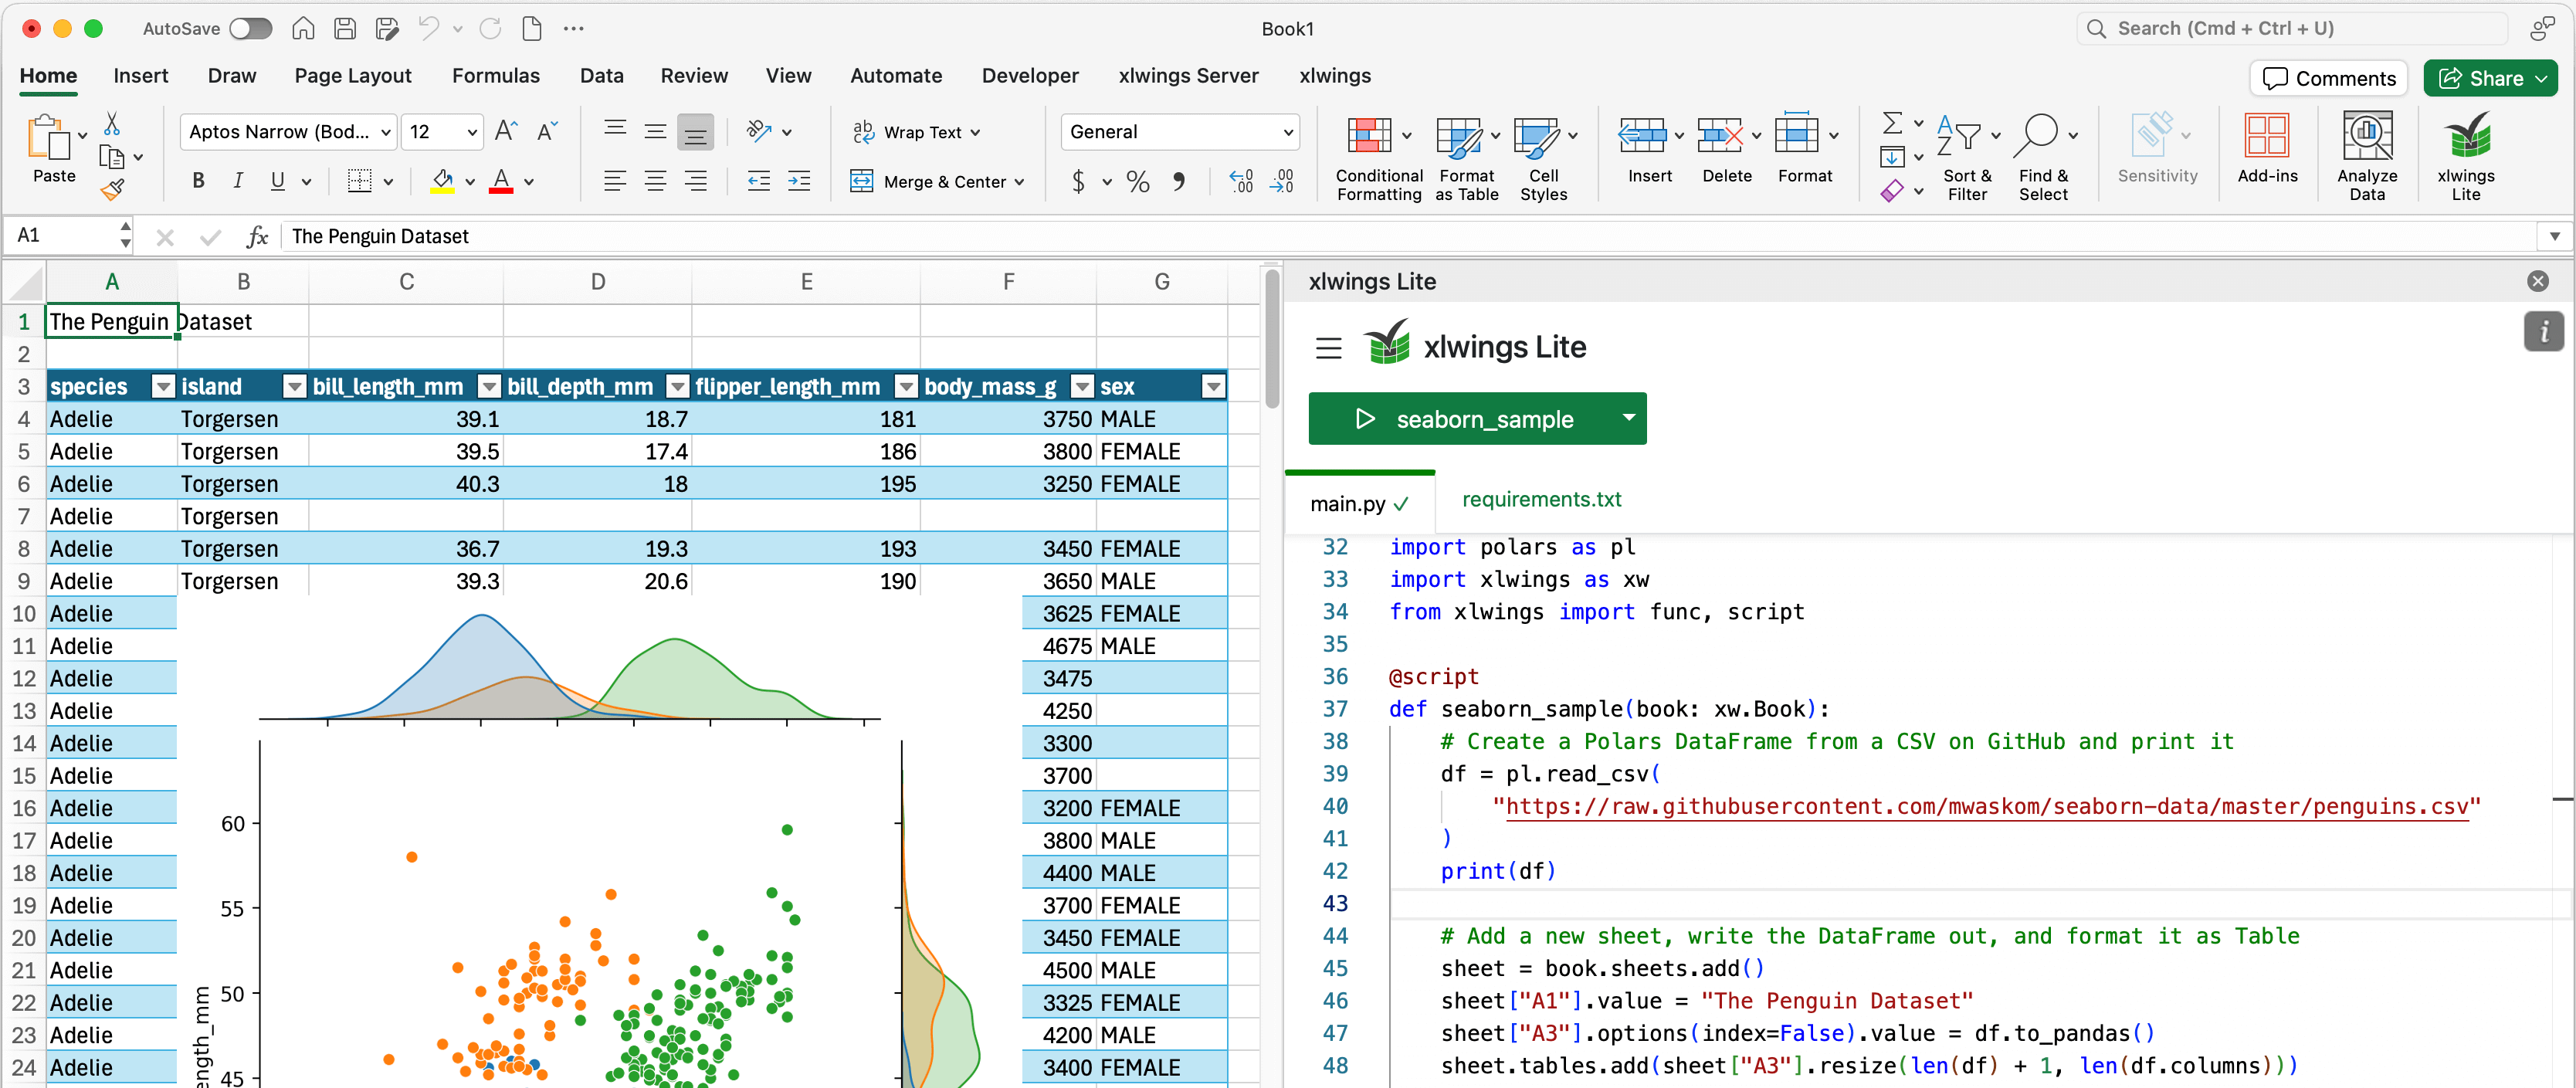
\includegraphics[width=1\textwidth]{wings.png}
\end{frame}


%\begin{frame}
%\frametitle{Компоненты системы}
%\framesubtitle{Структура взаимодействия компонентов системы}
%\begin{figure}[h]
%\includegraphics[width=9cm,height=5cm,keepaspectratio]{service-comp.pdf}
%\end{figure}
%\end{frame}

\begin{frame}
\frametitle{Обработка запроса}
\framesubtitle{последовательность обмена информацией для~выполнения команды}
    \centering
    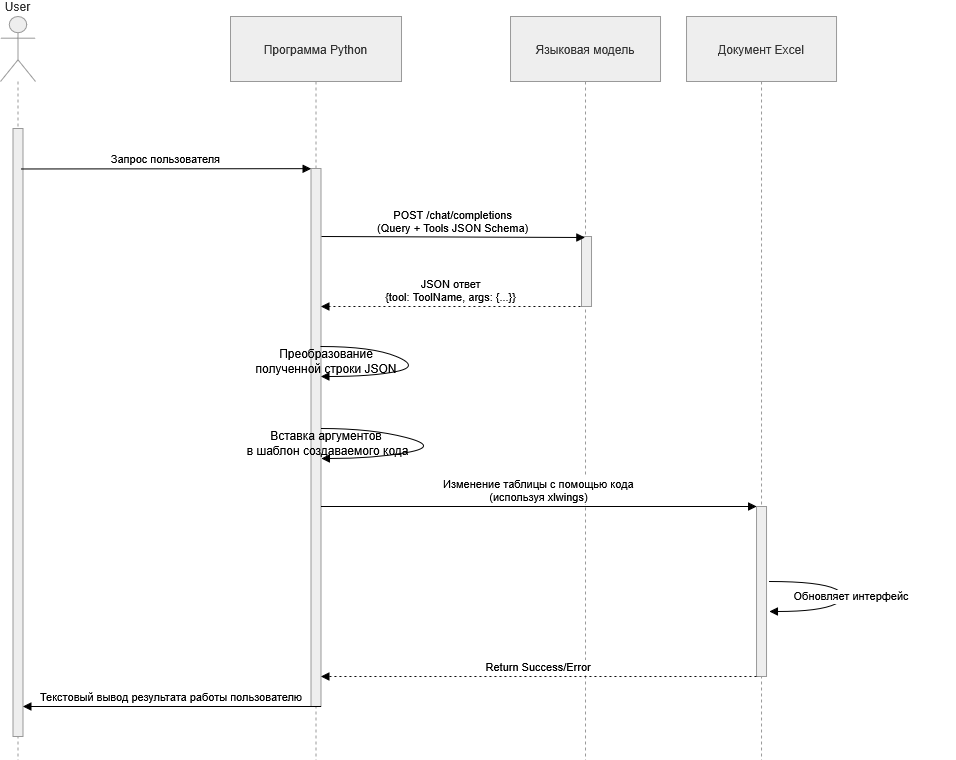
\includegraphics[width=0.9\textwidth]{sequencediagram.png}
\end{frame}

\begin{frame}{Основные инструменты}
    \scriptsize
    \setlength{\tabcolsep}{3pt}
    \renewcommand{\arraystretch}{0.85}
    \centering
    \begin{tabular}{|p{0.32\textwidth}|p{0.4\textwidth}|p{0.25\textwidth}|}
        \hline
        \textbf{Название инструмента} & \textbf{Описание} & \textbf{Аргументы} \\
        \hline
        \texttt{write\_cell} & Записывает заданное значение в указанную ячейку. & \texttt{cell\_coord}, \texttt{cell\_value} \\
        \hline
        \texttt{edit\_text\_format} & Изменяет стиль шрифта (жирный, курсив, подчеркивание) для диапазона. & \texttt{target\_range}, \texttt{format\_type}, \texttt{status} \\
        \hline
        \texttt{change\_cell\_color\_rgb} & Изменяет цвет заливки фона диапазона. & \texttt{target\_range}, \texttt{rgb\_values}, \texttt{clear\_color} \\
        \hline
        \texttt{highlight\_matching\_rows} & Выделяет цветом строки, соответствующие определенному условию. & \texttt{range\_address}, \texttt{filter\_col}, \texttt{operator}, \texttt{value}, \texttt{highlight\_color} \\
        \hline
        \texttt{create\_excel\_chart} & Создает диаграмму в формате Excel на основе диапазона данных. & \texttt{chart\_type}, \texttt{data\_range}, \texttt{title}, \texttt{location} \\
        \hline
        \texttt{find\_and\_replace} & Выполняет массовую замену текста в определенном диапазоне или столбце. & \texttt{target\_range}, \texttt{find\_text}, \texttt{replace\_text}, \texttt{match\_entire\_cell} \\
        \hline
        \texttt{remove\_duplicates} & Очищает таблицу, удаляя дубликаты строк на основе критериев столбца. & \texttt{table\_range}, \texttt{columns\_to\_check}, \texttt{has\_headers} \\
        \hline
    \end{tabular}
\end{frame}

\begin{frame}[allowframebreaks]
\frametitle{Пример использования}
\framesubtitle{Без интеллектуального ассистента}
    \begin{itemize}
    \item \textbf{Задание}: выделить строки валют с курсом больше 80.

    \item \textbf{Действия пользователя}:
    \end{itemize}
    \begin{enumerate}
  \item {
Выделить диапазон
  }
  \item {
Создать новое правило условного форматирования 
 }
    \vspace{0.5cm}

    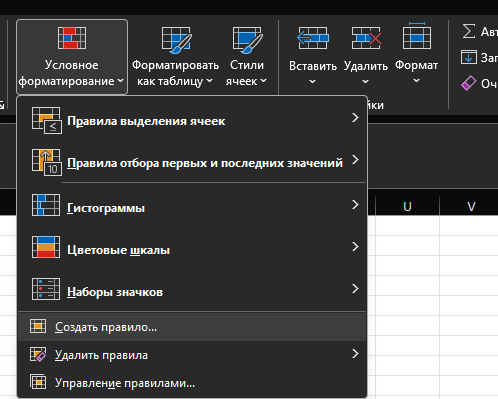
\includegraphics[width=0.5\textwidth]{highlightmanual1.png}
        \vspace{0.5cm}

    \item Настроить формулу - указать столбец сравниваемых значений и сравнение
    \item Настроить формат - заливка и ее цвет
\end{enumerate}
    \centering
    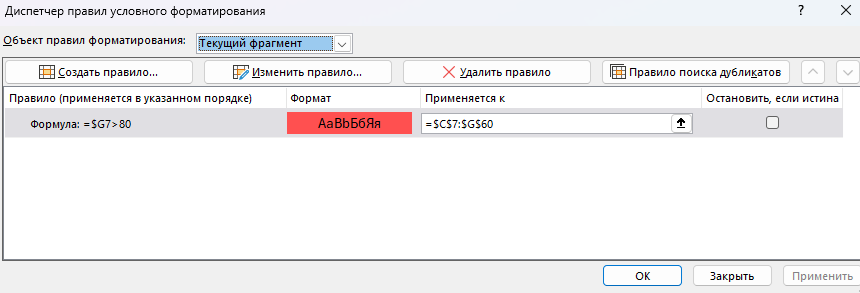
\includegraphics[width=1\textwidth]{highlightmanual2.png}
\end{frame}

\begin{frame}[fragile]
\frametitle{Пример использования III}
\framesubtitle{С интеллектуальным ассистентом}

\begin{enumerate}
    \item
    Запрос:
    
    Выдели все строки, в которых \textcolor{green}{Курс} \textit{больше} \textcolor{purple}{80} \textcolor{red}{светло-красным цветом}.
    Таблица начинается в ячейке \textcolor{blue}{C6}

    \item
    Ответ LLM:
\begin{Verbatim}[commandchars=\\\{\}]
Tool Name: highlight_matching_rows
Arguments String:
(\textcolor{blue}{"range_address":"C6"},\textcolor{green}{"filter_col":"Курс"},
 \textit{"operator":">"},\textcolor{purple}{"value":"80"},
\textcolor{red}{"highlight_color":[255,192,203]})
\end{Verbatim}
   \item
    Использование шаблона highlight\_matching\_rows для выполнения функции с использованием полученных аргументов. 
\end{enumerate}
\end{frame}  

  \begin{frame}
\frametitle{Результат работы ассистента}
\framesubtitle{Ассистент покрасил строки валют с курсом выше 80}

    \centering
    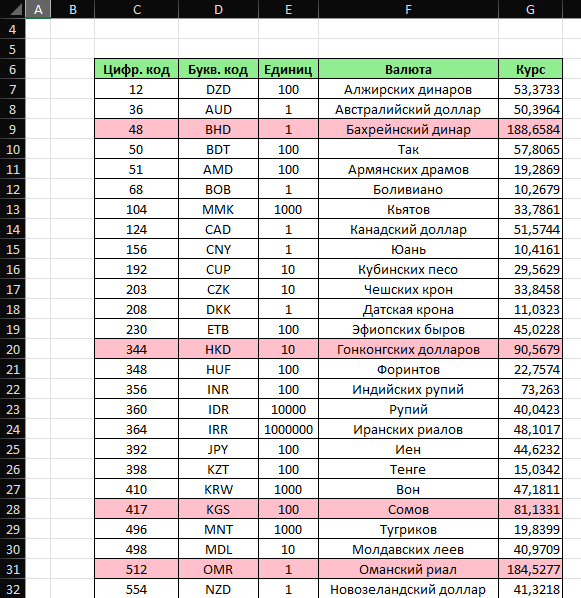
\includegraphics[width=0.8\textwidth]{highlightresult.png}
\end{frame}  

\begin{frame}
\frametitle{Сравнение языковых моделей}
\framesubtitle{При вызове инструмента highlight\_matching\_rows}

\small

\textbf{Запрос:} Покрась все строчки, в которых значение Курс больше, чем курс доллара к рублю в 2020. Таблица начинается в C6

\vspace{0.8em}

\centering
\renewcommand{\arraystretch}{1.35}
\begin{tabular}{|p{0.17\textwidth}|p{0.33\textwidth}|p{0.12\textwidth}|p{0.13\textwidth}|p{0.15\textwidth}|}
    \hline
    \textbf{Модель} & \textbf{Описание модели} & \textbf{Время работы} & \textbf{Аргумент Value} & \textbf{Стоимость в валюте BotHub*} \\
    \hline
    \texttt{claude sonnet-4.5} & {Мощная современная модель} & 2.71 с & 73 & 3944 \\
    \hline
    \texttt{gpt-4o-mini} & Малая модель прошлого поколения & 1.51 с & 2020 & 63 \\
    \hline
    \texttt{gemini-3.1 flash-lite} & Быстрая модель нового поколения & 2.45 с & 75 & 973 \\
    \hline
\end{tabular}

\vspace{0.7em}

{\footnotesize *5000 BotHub Caps $\approx$ 1 рубль}

\end{frame}

\begin{frame}
  \frametitle{Заключение}
  \framesubtitle{Текущие результаты работы}

  \begin{enumerate}
  \item {
Разработан интеллектуальный ассистент для~управления Microsoft Excel с~обработкой запросов на~естественном языке. 
  }
  \item {
Организовано взаимодействие с~языковыми моделями при~помощи OpenAI~API.
  }
  \item {
Работа ассистента протестирована на~проверочных примерах с~получением планируемого результата.
    }
   \item {
Произведено сравнение работы ассистента при использовании различных языковых моделей.
    }
    \end{enumerate}
\end{frame}

\begin{frame}
  \begin{center}
{\Large Спасибо за~внимание!}
    \end{center}
  \end{frame}
   
\end{document}
